\chapter{Analyse fonctionnelle}

\section{Interview}

Après notre interview avec notre encadrant Ali Mansour, nous avons réalisé un tableau des spécifications suivantes:

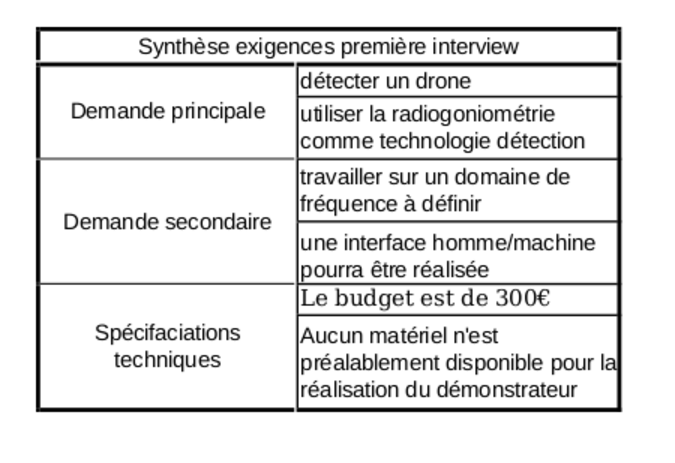
\includegraphics[width=0.8\textwidth]{interview}


\section{Tableau des spécifications}
En prennant en compte les recommandations de notre encadrant, et les recherches qu nous avons réalisées, nous avons établie les contraintes et les spécifications suivantes:

%\includegraphics[width=\textwidth]{tableauSpe}
\includepdf{./images/tableauSpe.pdf}

%Compte tenu des recherches que nous avons réalisées, nous avons établi l'étude fonctionnelle suivante.

%De la synthèse de ce tableau découle le diagramme Pieuvre et les SADT suivant.

\section{Diagramme pieuvre}

\hspace{-2cm}
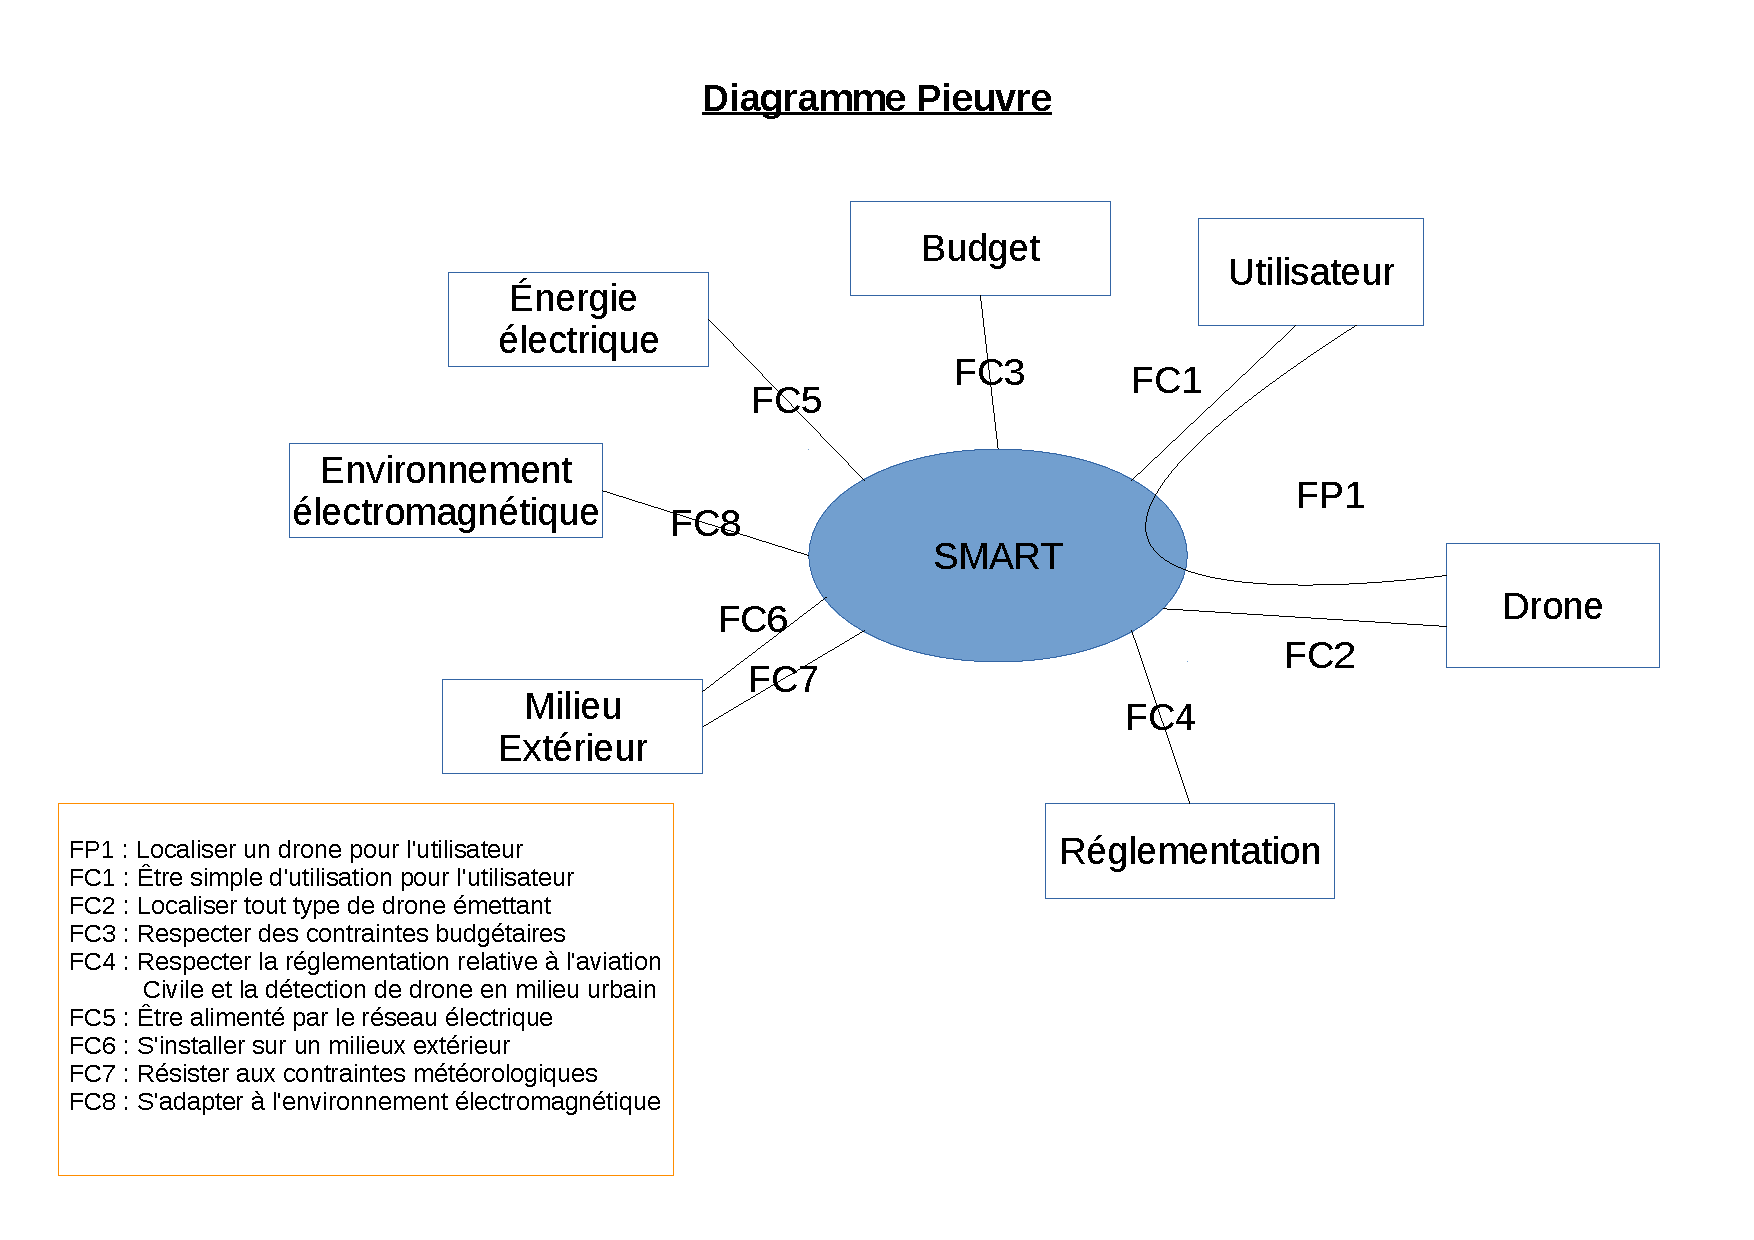
\includegraphics[width=1.18\textwidth]{Diagramme_pieuvre.pdf}
\captionof{figure}{Diagramme pieuvre}



\section{SADT}

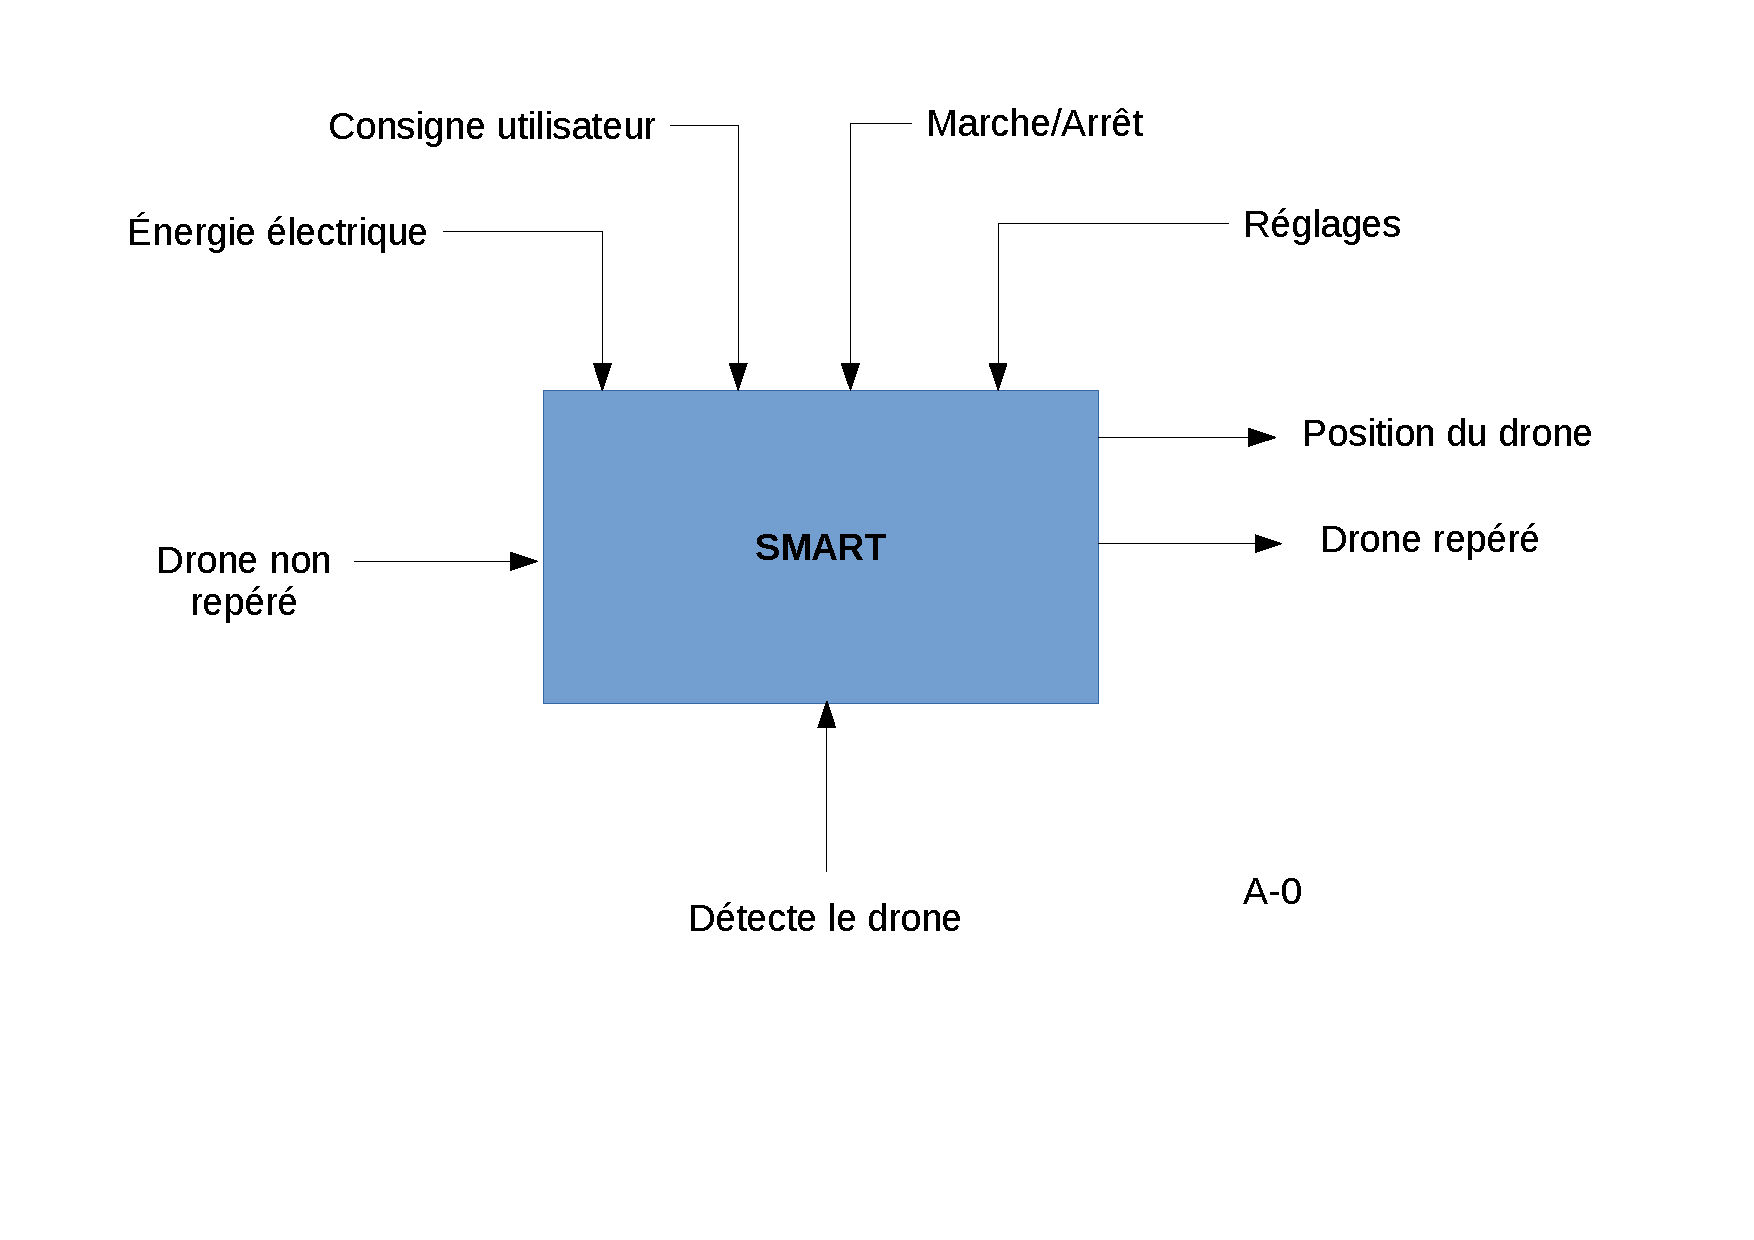
\includegraphics[width=\textwidth]{SADT_A-0.pdf}
\captionof{figure}{SADT A-0}
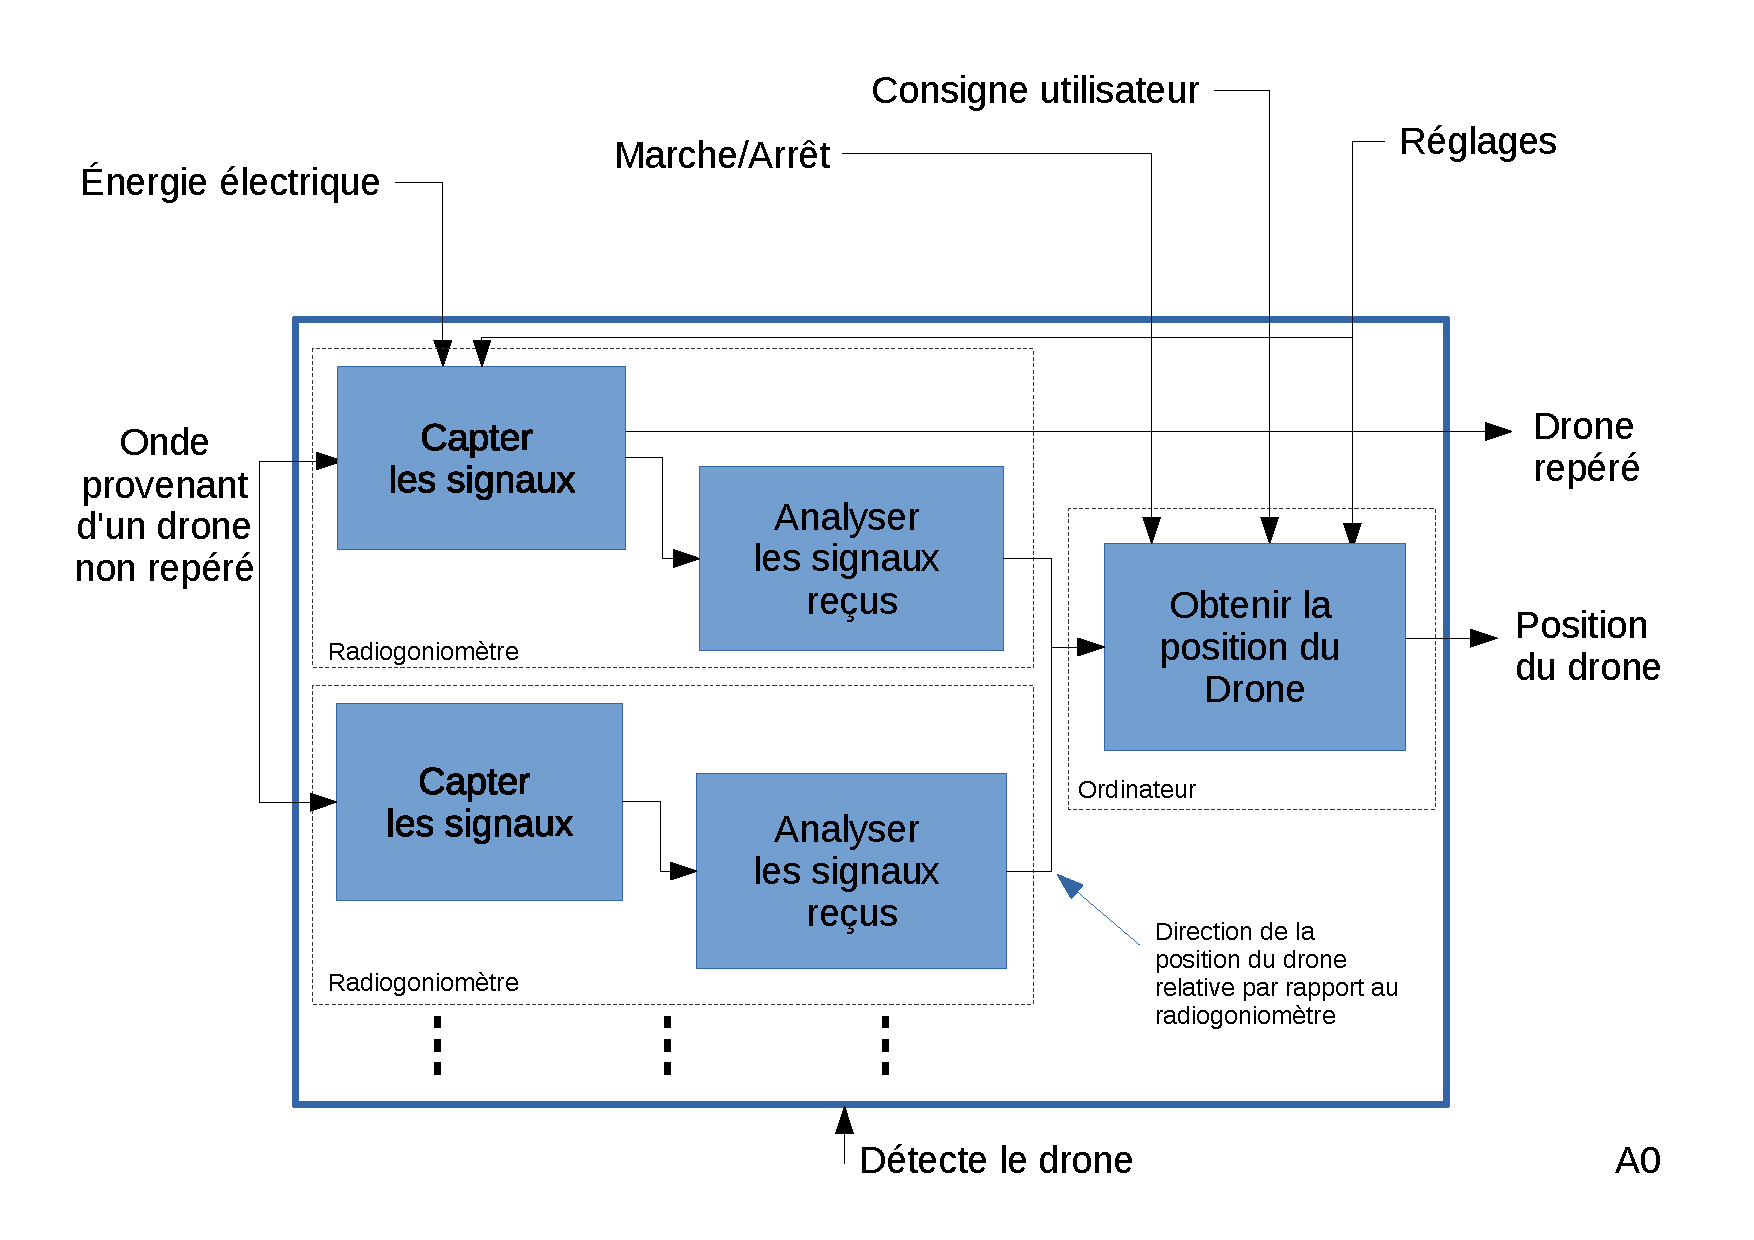
\includegraphics[width=\textwidth]{SADT_A0.pdf}
\captionof{figure}{SADT A0}

\parindent=15pt

Comme on peut le voir sur le SADT A0, nous avons découpé notre objectif en trois parties.

Dans un premier temps il faut capter les signaux. Pour cela il faut réaliser un balayage sur le radiogoniomètre pour détecter les bons signaux.

Ensuite, il faut analyser les signaux reçus pour s'assurer que nous sommes bien en présence d'un drone.

Enfin, il faut récupérer les données des radiogoniometres pour déterminer la position du drone.







%%% Local Variables: 
%%% mode: latex
%%% TeX-master: "rapport_analyse"
%%% End: 
